% !TeX program = lualatex
\documentclass[tikz,border=2pt]{standalone}

\usepackage{pgfplots}
\pgfplotsset{compat=1.18}
\usetikzlibrary{shapes.geometric,backgrounds}
\usepgfplotslibrary{fillbetween}
\usepackage[colorlinks=true,linkcolor=blue,urlcolor=blue]{hyperref}

% Opaque white ground: the SVG may be displayed on pages that use a dark theme,
% where a transparent background would swallow the black axes and labels.
\pagecolor{white}

\begin{document}

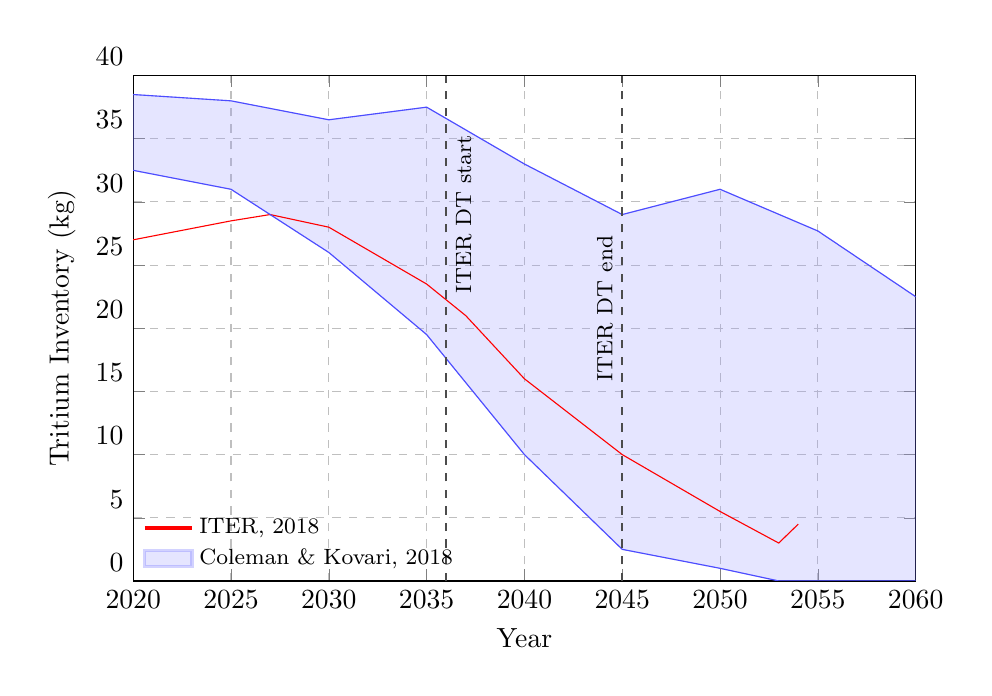
\begin{tikzpicture}[show background rectangle,
inner frame sep=4pt,
background rectangle/.style={fill=white, draw=none}]
\begin{axis}[
  width=0.95\linewidth,
  height=8.0cm,
  xmin=2020, xmax=2060,
  ymin=0, ymax=40,
  xlabel={Year},
  ylabel={Tritium Inventory (kg)},
  grid=both,
  legend style={at={(0.00,0.00)},anchor=south west,draw=none,fill=none,align=left},
  legend cell align={left},
  line width=1.2pt,
  xtick={2000,2005,2010,2015,2020,2025,2030,2035,2040,2045,2050,2055,2060},
  xticklabels={2000,2005,2010,2015,2020,2025,2030,2035,2040,2045,2050,2055,2060},
  ytick={0,5,10,15,20,25,30,35,40},
  scaled ticks=false,
  major grid style={dashed,gray!50},
  %xticklabel style={rotate=0,anchor=north west}
  yticklabel style={rotate=0,anchor=south east}
]

% ITER, 2018 (red)
\addplot+[color=red,mark=none]
  coordinates {
    (2020,27) (2025,28.5) (2027,29) (2030,28) (2035,23.5) (2037,21) (2040,16) (2045,10) (2050,5.5) (2053,3) (2054,4.5)
  };
\addlegendentry[font=\footnotesize]{ITER, 2018}

% Upper bound (max) path for global supply band
\addplot+[draw=blue!70, mark=none, name path=upper, forget plot]
  coordinates {
    (2020,38.5) (2025,38.0) (2030,36.5) (2035,37.5) (2040,33) (2045,29) (2050,31) (2055,27.7) (2060,22.5)
  };

% Lower bound (min) path for global supply band
\addplot+[draw=blue!70, mark=none, name path=lower, forget plot]
  coordinates {
    (2020,32.5) (2025,31) (2030,26) (2035,19.5) (2040,10) (2045,2.5) (2050,1) (2053,0) (2055,0) (2060,0)
  };

% Shaded fill between upper and lower (global supply range)
\addplot[
  fill=blue!40, draw=blue!70, opacity=0.25
] fill between[of=upper and lower];

\addlegendimage{area legend, fill=blue!40, opacity=0.25, draw=blue!70}
\addlegendentry[font=\footnotesize]{Coleman \& Kovari, 2018}

% =====================================================
% ITER D-T campaign vertical lines (2036-2045)
% =====================================================
\addplot[thick, dashed, color=black!70] coordinates {(2036,0) (2036,40)};
\addplot[thick, dashed, color=black!70] coordinates {(2045,0) (2045,40)};

% Optional text labels
\node[anchor=north west, rotate=90, font=\footnotesize, color=black]
  at (axis cs:2036,22) {ITER DT start};
\node[anchor=south west, rotate=90, font=\footnotesize, color=black]
  at (axis cs:2045,15) {ITER DT end};

\end{axis}
% fill between switches pgfplots to its own layer list; add 'background' so the
% white background rectangle has a layer to be drawn on.
\pgfsetlayers{background,axis background,axis grid,axis ticks,axis lines,axis tick labels,pre main,main,axis descriptions,axis foreground}
\end{tikzpicture}

\end{document}